\documentclass[conference]{IEEEtran}
\IEEEoverridecommandlockouts
\usepackage{cite}
\usepackage{amsmath,amssymb,amsfonts}
\usepackage{graphicx}
\usepackage{textcomp}
\usepackage{xcolor}
\usepackage{booktabs}
\usepackage{tabularx}
\usepackage{array}
\usepackage{float}
\usepackage{url}
\usepackage{caption}
\captionsetup{font=small,labelfont=bf}

\Urlmuskip=0mu plus 2mu\relax
\def\UrlBreaks{\do\/\do-\do\_\do\.\do\?\do\=\do\&}
\emergencystretch=2em

\graphicspath{{../results/presentation/}{../results/}}
\newcolumntype{Y}{>{\raggedright\arraybackslash}X}
\newcommand{\code}[1]{\texttt{\scriptsize #1}}
\newcommand{\pjbit}{pJ/bit}
\newcommand{\tbps}{Tb/s}
\newcommand{\figref}[1]{Fig.~\ref{#1}}
\newcommand{\tabref}[1]{Table~\ref{#1}}
\newcommand{\secref}[1]{Sec.~\ref{#1}}

\def\BibTeX{{\rm B\kern-.05em{\sc i\kern-.025em b}\kern-.08em
    T\kern-.1667em\lower.7ex\hbox{E}\kern-.125emX}}

\begin{document}

\title{Topology-Aware Mapping for Photonic Interconnects in TPU-Class LLM Accelerators}

\author{
\IEEEauthorblockN{Pranav Sitaraman}
\IEEEauthorblockA{\textit{MIT 6.5930} \\ sitaraman.pranav@gmail.com}
\and
\IEEEauthorblockN{Simone Surdi}
\IEEEauthorblockA{\textit{MIT 6.5930} \\ simonesurdi@gmail.com}
}

\maketitle

\begin{abstract}
We evaluate co-packaged photonic interconnect---using the public
Lightmatter Passage family (EVK50/EVK100/L200/L200X/M1000) as a concrete
reference point---as an emerging technology for TPU-class accelerator
clusters running large language model workloads. Because AccelForge does
not natively model an inter-chip network, we add (i) a topology-aware
network model with hop count, contention, multicast semantics, and
per-bit energy; (ii) an iterative feedback loop that folds the
network cost back into a logical cluster-memory level so that the
AccelForge mapper sees network-augmented memory; and (iii) an explicit
distributed-schedule layer above the mapper that enumerates
XLA/GSPMD-style policies (sharded collective, remote pooled-HBM
streaming, replicated cache, photonic multicast cache fill) and a
9216-chip Ironwood-class superpod stage model. Three insights stand
out. First, the intra-chip mapping (partitioning, dataflow, tile
sizing in the 6.5930 sense) is essentially invariant under photonics:
0/24 inner mapping signatures change in the TPU-cube study, while
5/16 distributed schedules change. The benefit therefore lives almost
entirely in a layer that the AccelForge mapper does not see. Second,
hardware multicast---not raw bandwidth---is the decisive property.
M1000 still outperforms a strong 3.5~\tbps{}, 6~\pjbit{} chiplet
baseline by 99.85\% on shared-state multicast. Third, the technology
is not a uniform multiplier. End-to-end inference reaches
14.50$\times$ latency speedup on a long-context Gemini-class proxy,
while training reaches only 1.43$\times$ because once collectives are
removed it becomes compute-dominated.
\end{abstract}

\section{Background, Related Work, and Motivation}
\label{sec:related}
Modern LLM systems are no longer limited only by matrix multiply
throughput. The hard part is moving activations, KV-cache state,
expert tokens, gradients, optimizer state, and shared weights through
a memory hierarchy that spans registers, on-chip buffers, HBM, and
thousands of accelerator chips. This is why the project is framed as
Project~12, ``evaluate a new technology,'' rather than as a simple
link replacement. The technology question is: if co-packaged
photonic interconnect is inserted into a TPU-class cluster, does it
only reduce the pJ/bit of an existing dataflow, or does it change the
mapping, memory placement, compiler schedule, and topology that a
large ML system should choose?

\subsection{AccelForge and optimal accelerator mapping}
AccelForge is the right base model because it treats accelerator
evaluation as a mapping problem. In the class vocabulary, a mapping
is not a vague schedule: it is the choice of partitioning,
dataflow/stationarity, tile sizing, and storage residency across the
memory hierarchy \cite{lec05-mapping,lec06-partitioning}. The recent
Turbo-Charged Mapper (TCM) paper sharpens that idea and is directly
relevant to how we interpret our results. TCM argues that accelerator
energy and latency depend on how computation and data movement are
scheduled, and that heuristic mappers can make hardware comparisons
misleading because they may miss the optimal mapping
\cite{tcm}. Its main addition is \emph{dataplacement}: which tensor
tiles are present at each memory level at a given time. In TCM's
terminology, dataplacement, dataflow, and tile shape together define
the mapspace; for a GPT-3 attention example, the paper reports a
space with 16 dataplacements, roughly $10^{15}$ dataflows, and
$10^{22}$ tile-shape choices, then prunes redundant and dominated
choices by up to 32 orders of magnitude \cite{tcm}. It also reports
optimal searches in feasible runtime and large EDP improvements over
prior heuristic or metaheuristic searches \cite{tcm}.

This matters for our project in two ways. First, we should not claim
that a new interconnect helps unless we give the mapper an
opportunity to respond. Second, if the AccelForge mapping does
\emph{not} move, that is still a meaningful result: it says the
local GEMM partitioning/dataflow/tile choice is dominated by
per-chip compute and local memory reuse, not by the fabric. Our
method therefore exposes a new logical memory level to AccelForge,
feeds network cost back into that level, and separately models the
compiler-level distributed schedule that AccelForge does not yet
represent.

\subsection{Google TPU clustering as the target architecture}
Google TPUs are the natural hardware target because their public
architecture already makes clustering a first-order design problem.
TPU v5p and TPU7x/Ironwood use high-speed inter-chip interconnect
(ICI), and TPU7x slices larger than 64 chips are constructed from
one or more $4{\times}4{\times}4$ cubes \cite{tpu7x,tpuv5p}. A full
TPU7x pod is documented at 9216 chips, with 2307 BF16 TFLOP/s and
4614 FP8 TFLOP/s per chip, 192~GiB HBM per chip, 7380~GiB/s HBM
bandwidth, and 1200~GB/s bidirectional ICI per chip
\cite{tpu7x}. Google also describes Ironwood as a system designed
for large inference workloads and as part of a co-designed AI stack
around hardware, XLA, and cluster management
\cite{ironwood-blog,hotchips-ironwood}.

Those facts shape the evaluation. The $4{\times}4{\times}4$ TPU
cube is the smallest realistic topology unit; the 9216-chip pod is
the scaling target; and compiler-visible sharding matters because
TensorFlow/JAX/XLA and PyTorch/XLA already present users with a
logical device abstraction and lower sharding annotations into
collectives \cite{xla-spmd}. Our report therefore treats the TPU
fabric as a memory-system problem, not as a black-box bandwidth
number. Node-to-node traffic corresponds to sharded activation or
collective-permute-like exchange; node-to-DRAM traffic corresponds
to remote HBM, KV, or optimizer-state fetch; shared-DRAM multicast
corresponds to cache-fill or weight/expert broadcast.

\subsection{Photonics and topology choices for future ML systems}
Photonics is relevant because future ML systems are becoming both
larger and more topologically sensitive. Electrical links work well
for short nearest-neighbor traffic, but a torus pays repeated hop
and fanout cost when data must cross a cube or broadcast to many
chips. Lightmatter's Passage family gives public points for the
kind of optical fabric we want to study. EVK100 is listed as a
3.2~\tbps{} aggregate link with 1.6~\tbps{} unidirectional
single-fiber transmission and a conservative 3.2~\pjbit{} target at
112G PAM4 \cite{lightmatter-evk100}; the broader Passage family
also reports a 1.9~\pjbit{} reference point used here as a
sensitivity case \cite{lightmatter-passage}. M1000 is listed at
114.6~\tbps{} aggregate bidirectional bandwidth and 2.3~\pjbit{}
including laser power \cite{lightmatter-m1000}. Lightmatter also
frames 3-D photonic interconnect as a way around the chip
``shoreline'' limit: electrical I/O exits through the package edge,
whereas a photonic interposer can expose far more communication
through the chip surface \cite{lightmatter-m1000}. The L200 family
and OCP co-packaged optics material provide additional public
references for switched optical fabrics \cite{lightmatter-l200,
lightmatter-ocp,lightmatter-tco}.

The architectural implication is that photonics is not just a better
wire. It changes the topology design space. A TPU-style system could
remain a torus with lower-energy optical links, but it could also
become a flatter switched fabric with hardware multicast, pooled
remote HBM, and different compiler placement choices. CiMLoop for
Photonics models photonic DNN accelerators at the component and
per-accelerator level \cite{ciml-photonics}; our project is
complementary because it keeps each chip's compute/memory hierarchy
fixed and asks how the inter-chip fabric changes the cluster-scale
mapping and schedule.

\subsection{Project question and contributions}
The report therefore studies whether Lightmatter-style photonics is
a constant-factor link substitution or a system-level change in how
LLM workloads should be mapped and scheduled. Three findings
summarize the answer.
\begin{enumerate}
    \item \textbf{The intra-chip mapping is stable; the distributed
    schedule changes.} For the 64-chip TPU cube, the AccelForge mapper
    converges to the same partitioning/dataflow/tile signature for all
    seven modeled interconnect technologies (0/24 inner signatures
    change). The benefit lives one layer above: the optimal
    distributed communication pattern flips for 5 of 16
    workload--scenario pairs, and the optimal compiler-visible
    schedule changes whenever multicast becomes available.
    \item \textbf{Hardware multicast, not raw bandwidth, dominates
    shared-state workloads.} A 3.5~\tbps{}, 6~\pjbit{} chiplet
    baseline is still beaten by M1000 by 99.85\% on shared-DRAM
    multicast traffic, because $N$ unicasts collapse into one logical
    broadcast. The same chiplet baseline is competitive on
    node-to-node activation exchange.
    \item \textbf{Photonics is not a uniform multiplier.} On a
    9216-chip Ironwood-class superpod, a long-context Gemini-class
    proxy reaches 14.50$\times$ inference latency speedup, but
    training only reaches 1.43$\times$. Once collectives shrink,
    training becomes compute-dominated; inference stays
    network-exposed because decode, KV attention, and MoE routing
    cross the fabric every step.
\end{enumerate}

What is novel here is the combination: AccelForge's inner mapper, a
topology cost model with multicast semantics, an enumeration of
compiler-visible distributed schedules, and a 9216-chip stage-level
superpod model are tied together into one reproducible evaluation.

\section{Network-Aware Architecture and Initial Tests}
\label{sec:approach}

\subsection{Connection to class concepts}
\label{sec:class-map}
The project is deliberately organized around the course vocabulary:
data movement dominates energy; memory hierarchy and locality control
reuse; mapping separates partitioning, dataflow, placement, and tile
sizing; and advanced technologies should be evaluated through the
changes they induce in the architecture model, not only through a
single headline device metric. \tabref{tab:class-map} gives the
concrete mapping from those concepts to the implementation.

\begin{table}[t]
\centering
\caption{How the report uses 6.5930 concepts.}
\label{tab:class-map}
\footnotesize
\begin{tabularx}{\linewidth}{lY}
\toprule
Class concept & Use in this project \\
\midrule
Data motion dominates &
Network, HBM, UB, register, and MAC energy are kept separate so the
result can say which level moves the joules. \\
Memory hierarchy &
\code{LogicalClusterMemory} sits above per-chip HBM; its cost is
updated with network energy/latency. \\
Mapping &
AccelForge reports partitioning, stationarity/dataflow, tile sizing,
and storage residency for each GEMM proxy. \\
Dataflow vs.\ schedule &
Intra-chip dataflow is the mapper's stationarity choice; the
distributed schedule is a compiler-level choice above AccelForge. \\
Calculating motion &
Logical-memory action counts are converted to bits, then priced by
topology, hop count, contention, and multicast semantics. \\
Advanced technology &
Photonics is evaluated as a system change in the L11 sense
\cite{lec11-advtech}: link energy, topology, multicast, pooled HBM,
and compiler-visible locality. \\
\bottomrule
\end{tabularx}
\end{table}

\subsection{Modeling stack: four layers}
\label{sec:stack}
A central source of confusion when evaluating new interconnects is
the word ``mapping.'' We separate the pipeline into four explicit
layers, only the first three of which live inside AccelForge.

\textbf{(1) Workload (einsum).}
\code{workload/single\_matmul.yaml} expresses
$O_{m,n}=\sum_k A_{m,k}W_{k,n}$ with rank sizes $(M,K,N)$ chosen
per LLM stage (decode MLP, KV attention, prefill projection,
long-context prefill, MoE dispatch, weight-gradient).

\textbf{(2) Architecture.}
\code{arch/tpu\_lightmatter\_cluster.yaml} declares
\code{!Memory}, \code{!Container}, and \code{!Compute} nodes:
\code{LogicalClusterMemory} (the cluster-wide pool whose
energy/latency we update from the network model), the
\code{NodeArray} fanout (\code{NodeX}/\code{NodeY}/\code{NodeZ}),
per-chip \code{HBM} (modeled at 7.03~\pjbit{} per
TPU v5p~\cite{tpuv5p}), \code{UnifiedBuffer}, the
\code{ProcessingElement} fanout with
\code{reuse\_input}/\code{reuse\_output}, a weight \code{Register},
and the \code{MAC}.

\textbf{(3) Mapping (AccelForge mapper output).} For a fixed
workload and architecture, AccelForge enumerates valid
\code{!Storage}/\code{!Temporal}/\code{!Spatial}/\code{!Compute}
sequences. A mapping therefore specifies, per loop variable, tile
shape, temporal-vs-spatial binding, and which fanout/storage level it
binds to. This is exactly the 6.5930 mapping
formalism~\cite{lec05-mapping,lec06-partitioning}: partitioning,
dataflow (stationarity), and tile sizing. Our \code{mapping\_signature}
encodes the spatial fanout assignments, memory residency, and action
counts that distinguish two mappings.

\textbf{(4) Distributed schedule (above AccelForge).} AccelForge has
no concept of how data moves \emph{between} cluster nodes. We add
three constructs above it: a \code{COMM\_PATTERN} parameter that
selects which tensor is resident in
\code{LogicalClusterMemory} versus per-chip \code{HBM} (so the mapper
sees a different architecture per pattern); the topology cost model
of \secref{sec:network}; and a discrete enumeration of named
XLA/GSPMD-style schedules: \texttt{xla\_spmd\_collective},
\texttt{remote\_hbm\_streaming}, \texttt{replicated\_hbm\_cache},
\texttt{photonic\_multicast\_cache}. The mapper does not pick among
these; we evaluate each analytically and report the best.

When this paper says ``dataflow,'' we mean the intra-PE stationarity
pattern in the class sense. When we say ``distributed dataflow
strategy'' or ``compiler schedule,'' we mean the layer-4 inter-chip
communication policy. These are different and we report them
separately.

\subsection{Topology cost model}
\label{sec:network}
For traffic of \(B\) bits over a topology with average hop count
\(h\), per-link energy \(e_\ell\), router latency \(t_r\), and link
bandwidth \(BW_\ell\):
\[
E_{\text{net}} = B \cdot h \cdot e_\ell, \quad
T_{\text{net}} = \frac{B}{BW_\ell / C(N)} + h \cdot t_r,
\]
where \(C(N)\) is the contention factor: \(C(N)=\sqrt{N}\) for a 2-D
mesh, \(\sqrt[3]{N}\) for a 3-D torus, and \(1\) for an optical
crossbar/switched fabric. Multicast semantics matter: a
non-multicast technology pays the unicast volume $N$ times for an
$N$-way fanout, while a multicast-capable photonic technology pays
only the unique payload once. This is why a flat switched optical
fabric can deliver gains far beyond what its raw bandwidth ratio
would predict.

\subsection{Iterative feedback loop (M1, M2, M3)}
\label{sec:iter}
AccelForge has no first-class NoC primitive between two storage
levels. Rather than fake the inter-chip ICI as an opaque
\code{!Memory}, we keep the network model explicit and feed it back
into \code{LogicalClusterMemory}:
\begin{enumerate}
    \item Run AccelForge with the current logical-memory energy and
    latency.
    \item Extract logical-memory read/write traffic from the best
    mapping.
    \item Evaluate the topology cost
    (\(E_{\text{net}}, T_{\text{net}}\)).
    \item Add the per-bit network cost to
    \code{LOGICAL\_READ\_ENERGY}/\code{LOGICAL\_WRITE\_ENERGY} and
    matching latencies.
    \item Re-run the mapper until the energy and signature
    stabilize.
\end{enumerate}
This realizes Milestones M1 (topology + logical-memory model),
M2 (iterative feedback), and M3 (improved topology proposal:
EVK100 optical crossbar and M1000 switched fabric) in one loop.

\subsection{Initial 16-node cluster tests}
\label{sec:initial}
The first experiment is deliberately small: a 16-node cluster with
the same accelerator node and workload, comparing an electrical
$4{\times}4$ mesh against an EVK100-class optical crossbar. The goal
is not to claim a final TPU result; it is to check whether the model
responds to the right traffic patterns. We test three cases. In
\texttt{node\_to\_node}, activations move between neighboring nodes.
In \texttt{node\_to\_dram}, one node fetches remote state through the
logical cluster memory. In \texttt{shared\_dram\_multicast}, one
payload fans out to many nodes, representing shared weight, expert,
or KV-cache fill.

This small test already shows the intended asymmetry. Node-to-node
traffic gains little because the electrical mesh is already close to
the data and the transfer can often hide behind compute. Remote and
multicast traffic benefit much more: the best 16-node EVK100 cases
reduce energy by 72.21\% and latency by 97.57\%. This is the sanity
check for the rest of the report. Photonics should not be sold as a
universal multiplier; it should help most when memory placement and
fanout dominate the cost.

\section{Scaling to TPU Cubes, Compiler Policies, and Superpod Workloads}
\label{sec:scaling}

\subsection{Scaling path}
\label{sec:scaling-path}
After the 16-node sanity check, we increase the model in four steps.
First, we replace the logical cluster with a TPU-style
$4{\times}4{\times}4$ cube and compare electrical torus ICI against
photonic torus and switched-fabric variants. Second, we ask whether
the best \texttt{COMM\_PATTERN} changes when the cube is priced with
photonic costs. Third, we add the compiler-visible schedule layer:
conventional sharded collectives, remote pooled-HBM streaming,
replicated HBM caching, and photonic multicast cache fill. Fourth,
we sweep from one cube toward the 9216-chip pod and compare against
a stronger advanced-chiplet baseline. This sequence keeps the
model auditable: each larger experiment adds exactly one modeling
idea on top of the previous one.

\subsection{Superpod stage model}
\label{sec:stage}
For the 9216-chip end-to-end study each LLM stage decomposes into
\begin{align}
T_{\text{stage}} &=
\max(T_{\text{compute}}, T_{\text{HBM}})
  + (1-\alpha_{\text{ovl}})\,T_{\text{net}},
\nonumber\\
E_{\text{stage}} &=
E_{\text{compute}}+E_{\text{HBM}}+E_{\text{net}}.
\nonumber
\end{align}
The overlap factor $\alpha_{\text{ovl}}\!\in\![0,1]$ models how much
network transfer is hidden behind compute and HBM. Modeled stages
include prefill, decode KV attention, decode weight/expert refill,
inference MoE dispatch/combine, training forward/backward, gradient
synchronization, training MoE traffic, and optimizer-state traffic.

\subsection{Experiment setup}
\label{sec:setup}
\textbf{Constants held fixed.} All comparisons keep compute (MAC array,
register, UB), per-chip HBM, and HBM energy/latency identical. Only
interconnect technology, topology, and distributed schedule change.
\tabref{tab:tech} lists the modeled technologies.

\begin{table}[t]
\centering
\caption{Modeled interconnect technologies. Bandwidth is per-link
one-way unless noted. Sources cited in \secref{sec:related}.}
\label{tab:tech}
\scriptsize
\setlength{\tabcolsep}{2pt}
\begin{tabularx}{\linewidth}{lrrcY}
\toprule
Technology & BW & Energy & MC & Role \\
\midrule
Electrical 800G       & 0.8~\tbps  & 10.0~\pjbit & --- & Electrical ICI baseline \\
Advanced chiplet      & 3.5~\tbps  & 6.0~\pjbit  & --- & Strong packaging baseline \\
Lightmatter EVK50     & 0.8~\tbps  & 4.6~\pjbit  & yes & SC25 demo~\cite{lightmatter-evk50} \\
Lightmatter EVK100    & 3.2~\tbps  & 3.2/1.9~\pjbit  & yes & Conservative / sensitivity \\
Lightmatter L200      & 16~\tbps   & 4.5~\pjbit  & yes & Switched fabric~\cite{lightmatter-l200} \\
Lightmatter L200X     & 32~\tbps   & 4.8~\pjbit  & yes & High-BW switched fabric~\cite{lightmatter-tco} \\
Lightmatter M1000     & 57.3~\tbps & 2.3~\pjbit  & yes & OCS full-stack study \\
\bottomrule
\end{tabularx}
\end{table}

\textbf{Baselines.} The 16-node experiment uses an electrical
$4{\times}4$ mesh; the 64-chip TPU cube uses a $4{\times}4{\times}4$
electrical torus (TPU v5p-class~\cite{tpuv5p}); the superpod uses an
Ironwood electrical torus (9216 chips, 4614 FP8 TFLOP/s per chip,
192~GiB HBM, 7.4~TB/s HBM bandwidth, 1200~GB/s bidirectional ICI per
chip~\cite{tpu7x}). The advanced chiplet baseline (3.5~\tbps{},
6~\pjbit{}) is included to rule out raw bandwidth as the only
explanation for photonic gains.

\textbf{Workloads.} AccelForge experiments use six GEMM proxies for
LLM stages with rank sizes drawn from public Gemini-class proxy
sizes; the superpod study uses three explicit proxies: dense Flash
(120B), sparse MoE Pro (4.7T total / 600B active, 32K context), and
long-context Deep Think (4.7T / 750B active, 131K context
\cite{gemini3,gemini3deepthink}). These are public stress points,
not claims about undisclosed Gemini 3/3.1 internals.

\textbf{Reproducibility.} All experiments run inside the
\texttt{accelforge:latest-amd64} Docker image via
\texttt{make study/notebook/test}. The 71-test unit/integration
suite verifies the technology catalog, network model, mapper loop,
artifact writers, and superpod summaries. CSV results and nine
presentation-ready figures are written under
\texttt{results/}.

\textbf{Threats to bias.} (i) Lightmatter values are public headline
numbers, so we modeled the architecture rather than a particular
product, and verified key constants against multiple public sources;
(ii) optical multicast is modeled optimistically as one logical
broadcast, neglecting laser sharing and switch reconfiguration;
(iii) the superpod stage model is analytical, not cycle-accurate;
(iv) Gemini parameter counts are unpublished, so we used proxy
workloads.

\section{Results and Discussion}
\label{sec:results}

\begin{figure}[t]
    \centering
    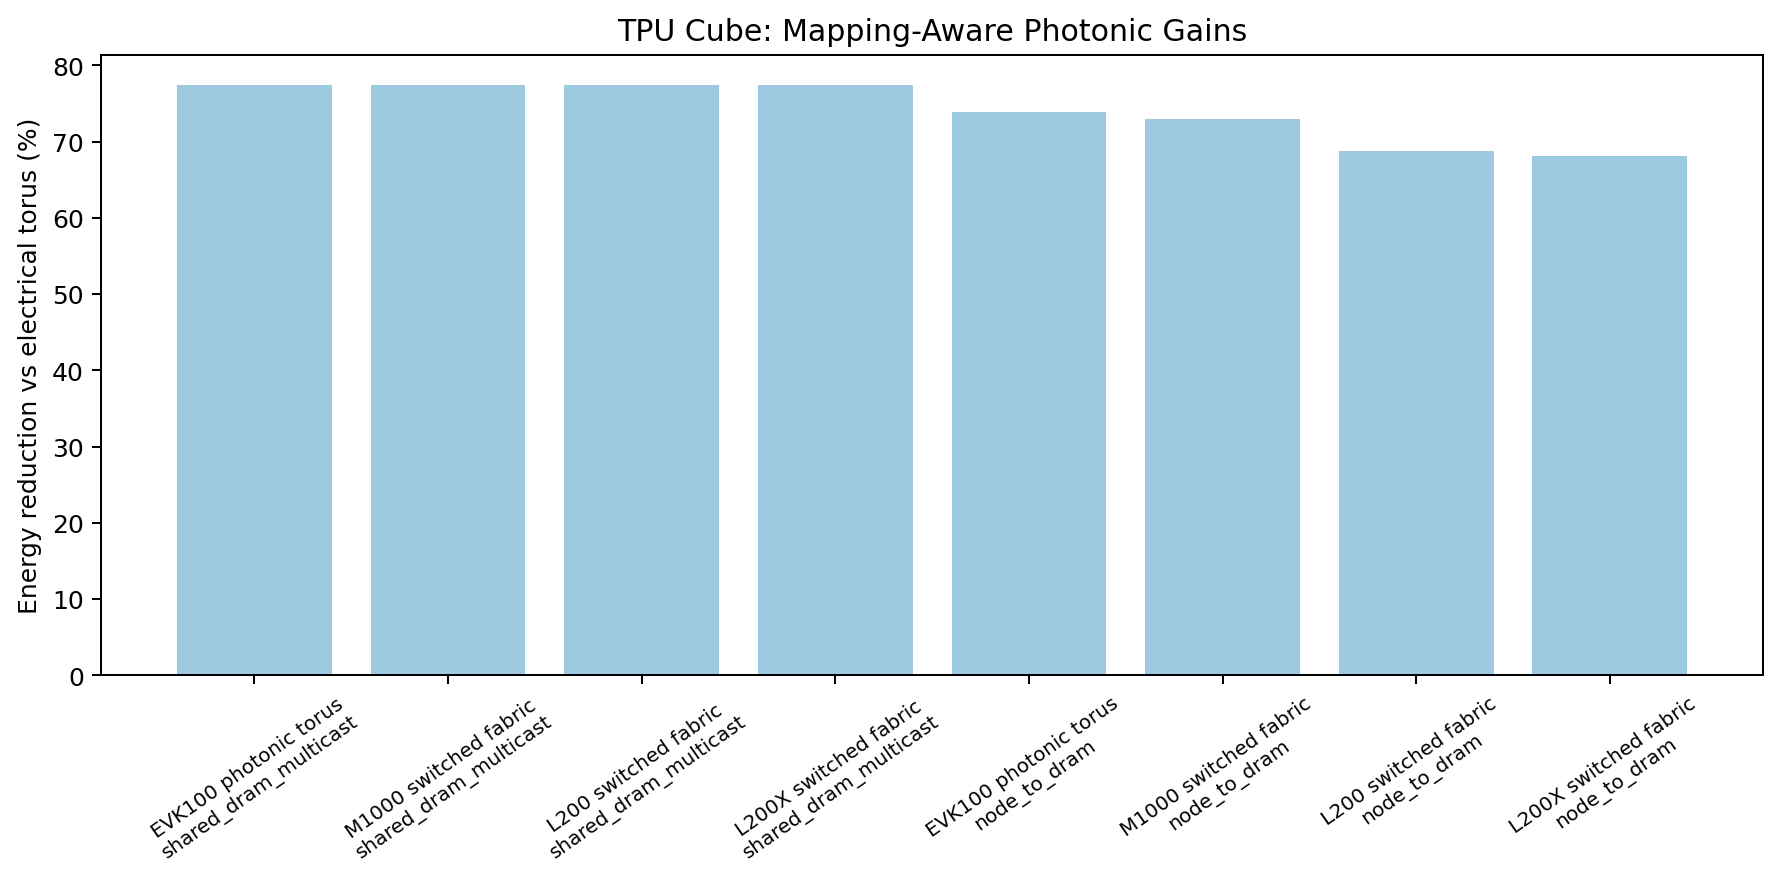
\includegraphics[width=0.96\linewidth]{02_tpu_mapping_reductions.png}
    \caption{TPU-cube AccelForge results. Energy and latency
    reductions for EVK100/L200/L200X/M1000 versus the
    $4{\times}4{\times}4$ electrical torus, by communication scenario.
    Multicast benefits the most; node-to-node exchange
    benefits least.}
    \label{fig:tpu-mapping}
\end{figure}

\begin{table}[t]
\centering
\caption{Headline results across the five evaluation axes.}
\label{tab:headline}
\footnotesize
\begin{tabularx}{\linewidth}{l l r Y}
\toprule
Axis & Metric & Value & Where \\
\midrule
16-node cluster & Energy red. & 72.21\% & EVK100 multicast \\
16-node cluster & Latency red. & 97.57\% & EVK100 multicast \\
TPU-cube net    & Energy red. & 99.91\% & M1000 multicast \\
TPU-cube map    & Energy red. & 77.70\% & M1000 KV attn \\
Inner mapping   & Changed     & 0/24    & TPU cube \\
Distributed map & Changed     & 5/16    & cluster \\
Compiler sched. & Best gain   & 67.75\% & M1000 stream \\
Scaling law     & Best slope  & 0.00    & M1000 multicast \\
Chiplet vs M1000& Energy red. & 99.85\% & multicast \\
Superpod inf.   & Speedup     & 14.50$\times$ & Deep Think \\
Superpod train. & Speedup     & 1.43$\times$ & Pro MoE \\
Superpod inf.   & Energy red. & 51.07\% & Deep Think \\
\bottomrule
\end{tabularx}
\end{table}

\subsection{The inner mapping is stable; the schedule changes}
\label{sec:result-stability}
The most surprising finding is the cleanly two-layered behavior of
photonics. Across 24 (workload, technology, scenario) combinations
on the 64-chip cube, the AccelForge mapper converges to the same
spatial fanout, residency, and action-count signature for all
photonic and chiplet variants---0 of 24 inner mappings change. This
is consistent with what we expect from class theory: the per-chip
loop nest is dominated by local compute and SRAM/HBM reuse
\cite{lec05-mapping,lec06-partitioning,lec03-memory}, and photonics
does not change those costs.

The benefit instead lives in two distinct layer-4 places.
\textbf{Distributed mapping (\code{COMM\_PATTERN}).} For 5 of 16
workload--scenario pairs, the optimal communication pattern flips
from node-to-node exchange to shared-DRAM multicast under EVK100 or
M1000, because the multicast volume cost has collapsed.
\textbf{Compiler schedule.} Among the four enumerated XLA/GSPMD-style
policies, the best policy switches whenever multicast becomes
available: \texttt{photonic\_multicast\_cache} dominates for
shared-state KV/expert refill, and \texttt{remote\_hbm\_streaming}
becomes attractive on M1000 for KV attention with a 67.75\% gain
versus the baseline policy.

This separation is not a modeling limitation; it is the actual answer
to ``does photonics change the mapping?''---the mapping is stable,
the schedule changes, and reporting them as one number would obscure
both. \figref{fig:compiler} visualizes the schedule changes.

\begin{figure}[t]
    \centering
    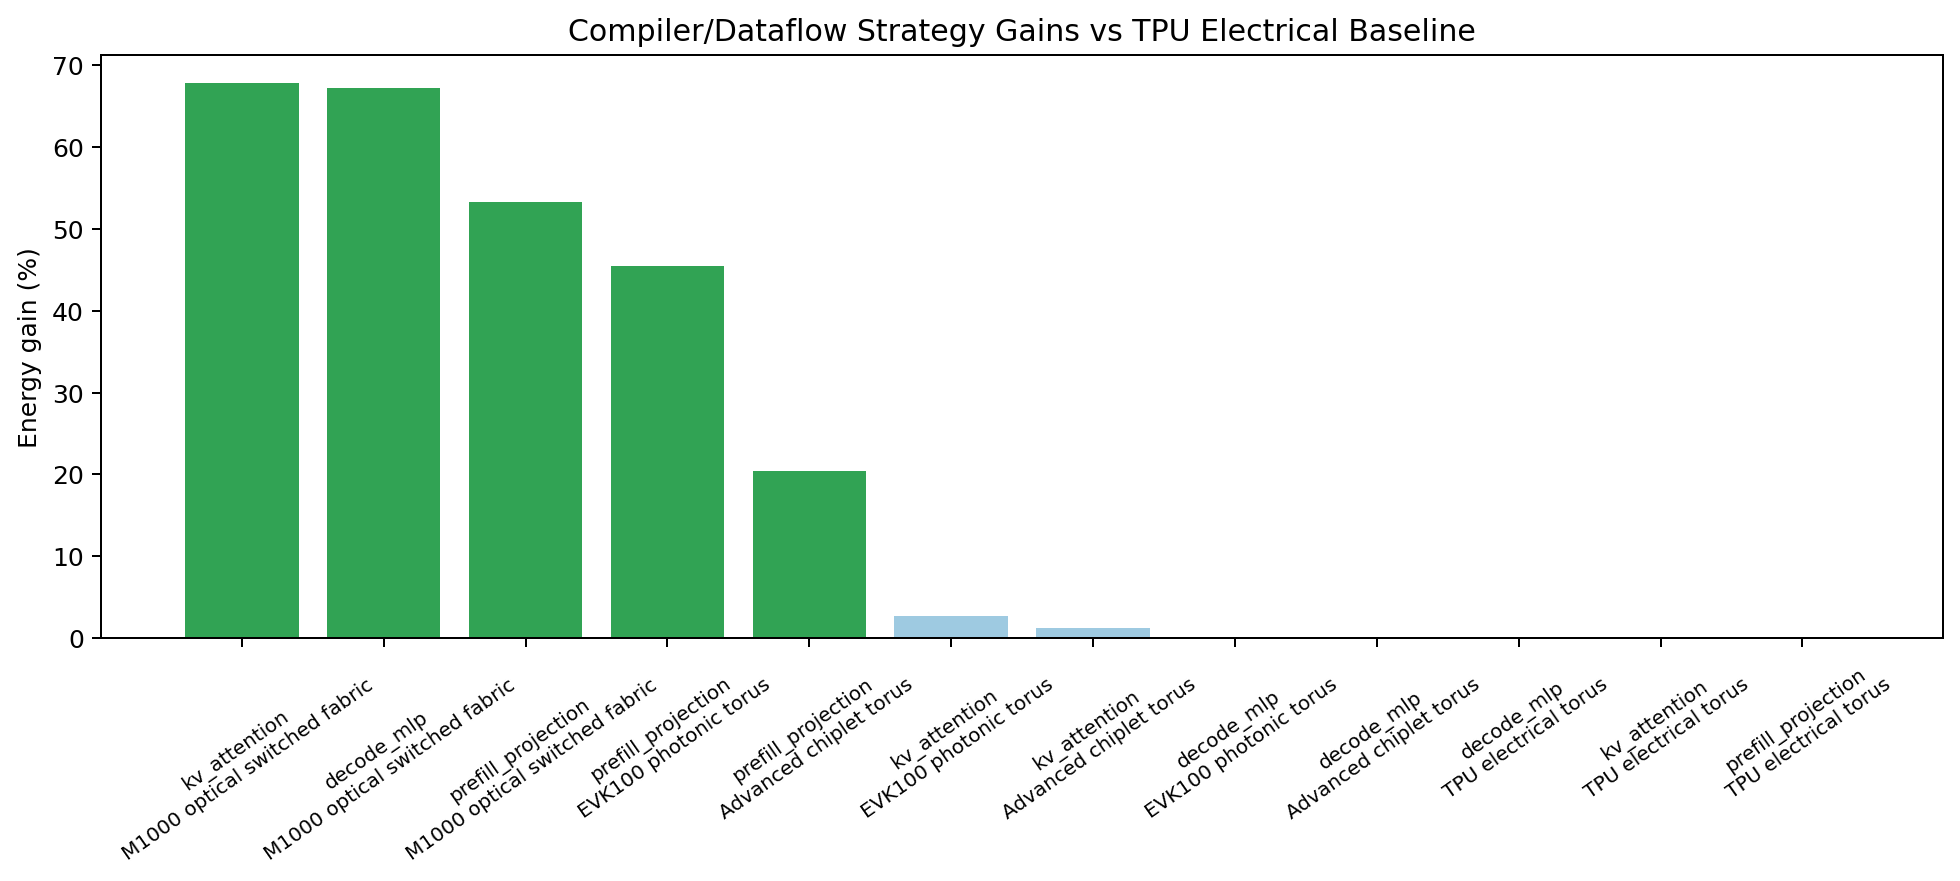
\includegraphics[width=0.96\linewidth]{04_compiler_strategy_choices.png}
    \caption{Best XLA/GSPMD-style schedule per workload and
    technology. Color-marked cases (e.g., M1000 KV attention) are
    where the optimal compiler-visible policy changes versus the
    electrical baseline.}
    \label{fig:compiler}
\end{figure}

\subsection{Multicast, not bandwidth, is decisive}
\label{sec:result-multicast}
The advanced chiplet baseline (3.5~\tbps{}, 6~\pjbit{}) was chosen
specifically to defeat the ``photonics just has more bandwidth''
hypothesis. On node-to-node activation exchange the chiplet baseline
is in fact close to EVK100. On shared-DRAM multicast the chiplet
baseline is beaten by M1000 by 99.85\%, because $N$ unicasts collapse
to one logical broadcast and contention disappears on a switched
fabric. This isolates hardware multicast as the architectural
property that matters most for shared-state LLM workloads (cache
fills, expert refill, weight broadcast). The flat
multicast scaling exponent (0.00 across the 64-to-9216-chip sweep)
makes the same point geometrically: torus and chiplet fabrics
accumulate hop and contention cost as $N$ grows; switched optical
multicast does not.

\subsection{Inference vs.\ training: not a uniform multiplier}
\label{sec:result-superpod}
\figref{fig:superpod} shows the end-to-end stage-decomposed result.
On the 9216-chip Ironwood-class superpod, the long-context Deep Think
proxy reaches 14.50$\times$ inference latency speedup with the full
M1000 photonic stack; the dense Flash-class proxy reaches a more
modest speedup; training reaches 1.43$\times$. The reason is exactly
what the stage model predicts: once collectives, MoE dispatch, and
KV broadcast traffic are removed, training becomes
compute-dominated---it spends most of its critical path inside
$\max(T_{\text{compute}}, T_{\text{HBM}})$, a term photonics does not
change. Inference, especially long-context inference, remains
network-exposed because decode is autoregressive and KV/expert
traffic must move every step. This is a positive prediction: future
TPU-class designs that pursue photonics for training payoff alone
will under-perform expectations; the strong case for photonics is
inference and long-context serving.

\begin{figure}[t]
    \centering
    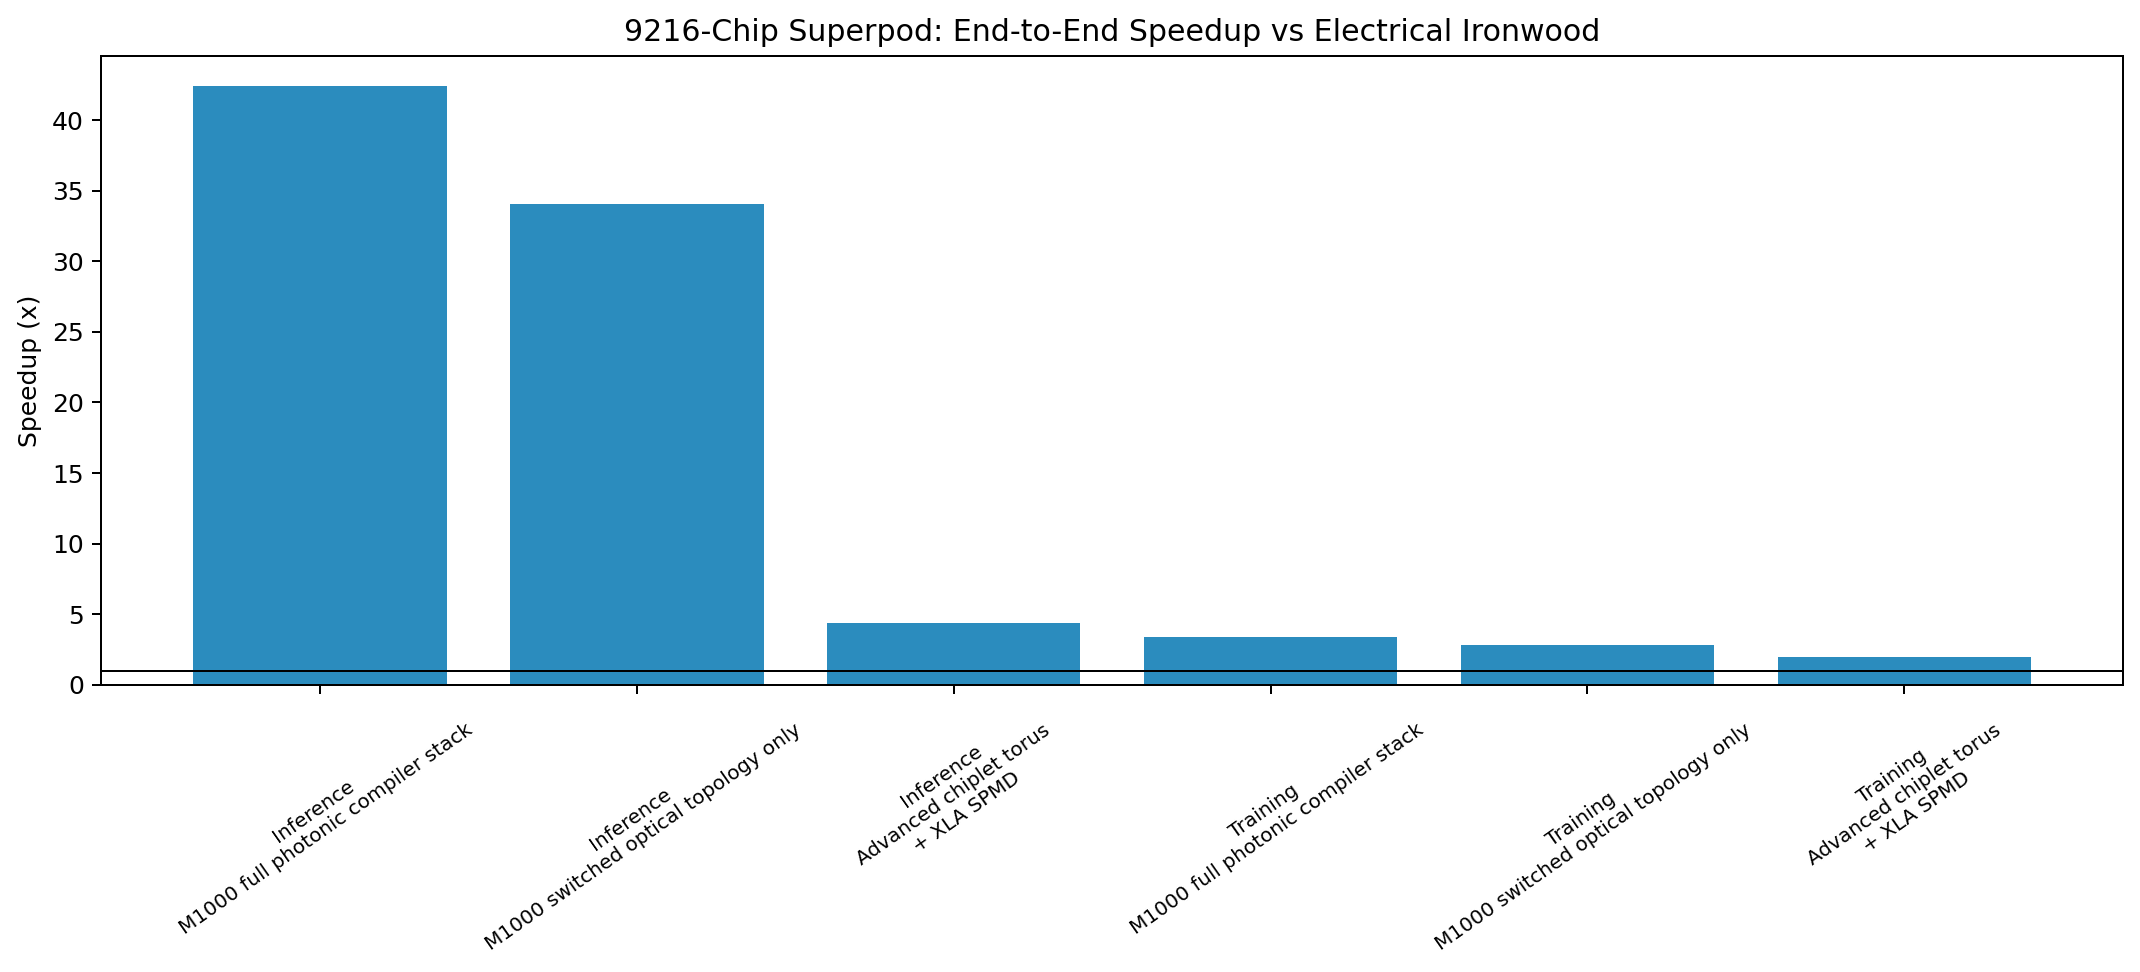
\includegraphics[width=0.96\linewidth]{07_superpod_end_to_end_speedups.png}
    \caption{End-to-end superpod speedups. Inference benefits much
    more than training; long-context inference benefits most.}
    \label{fig:superpod}
\end{figure}

\subsection{Where the approach helps and where it does not}
\label{sec:where}
\textbf{Beneficial.} (a) Long-context inference, where decode and
KV-attention traffic dominate the critical path. (b) Sparse-MoE
serving, where expert-parallel all-to-all traffic is network-bound.
(c) Pooled remote HBM access, where flat fabrics make remote
streaming competitive with replication. (d) Cache-fill /
weight-broadcast traffic, which exploits hardware multicast directly.

\textbf{Not beneficial.} (a) Local nearest-neighbor activation
exchange, where electrical torus is already efficient (one hop). (b)
Compute-dominated training stages, where $\max(T_{\text{compute}},
T_{\text{HBM}})$ dominates. (c) Workloads whose tile mapping is
already optimal under the electrical baseline---photonics does not
change those mappings.

\textbf{Limitations and future work.} The optical multicast model is
optimistic; a more detailed model would account for switch
reconfiguration, laser sharing, and wavelength conflicts. The
superpod stage model is analytical and uses an overlap factor;
cycle-accurate simulation would tighten the inference numbers. The
distributed-schedule enumeration is discrete; a continuous compiler
search (e.g., direct XLA integration) is the natural next step. The
proxy workloads bound real Gemini-class behavior but do not claim
exact correspondence.

\textbf{What worked vs.\ what did not.} Worked: the
iterative-feedback loop converged in $\le 3$ iterations on every
case; the topology model produced the predicted multicast
asymmetries; the superpod stage model reproduced the
inference-vs-training divergence cleanly. Did not work: trying to
make AccelForge model the inter-chip NoC directly via a degenerate
\code{!Memory} produced opaque, hard-to-debug numbers; we kept the
network model external instead. The inner mapping signature did
\emph{not} change under any photonic technology---an honest negative
result that we report rather than hide.

\textbf{Future work.} Direct XLA/Pallas integration; a
cycle-accurate optical-switch simulator; co-design of MoE expert
placement under photonic locality; extending the stage model to
training with pipeline parallelism and ZeRO-3 optimizer sharding.

\clearpage
\section{Reproducibility and Submission Checklist}
The submitted artifact is intended to be read in two ways. First, it
is a class project report: the paper, poster, and slide deck explain
the problem, the accelerator abstraction, the network equations, the
mapping results, and the limitations using the vocabulary of
6.5930. Second, it is an executable study: the repository contains
the AccelForge architecture file, the workload template, the network
and superpod analysis script, the notebook, and the regression tests
needed to reproduce the tables and figures.

The public technology constants in the model are cross-checked
against the cited primary sources. The class-specific pieces are
kept explicit: AccelForge supplies the einsum-to-memory-hierarchy
mapping, the project adds the logical-memory and topology-cost
feedback loop, and the distributed schedule layer captures
compiler-visible choices above the local tile mapping. All headline
results in \tabref{tab:headline} are regenerated by
\texttt{make study}; \texttt{make notebook} rebuilds and executes
the notebook; \texttt{make deliverables} compiles the report, slide
deck, poster, and summary sheet; and \texttt{make test} runs the
71-test validation suite. The checked results therefore come from
the same code path as the submission PDFs rather than from manually
edited tables.

\begin{thebibliography}{99}
\footnotesize

\bibitem{lec03-memory} V. Sze and J. Emer, ``Memory, Metrics, Einsums,
and Transformers,'' MIT 6.5930 lecture notes, Spring 2026.

\bibitem{lec05-mapping} V. Sze and J. Emer, ``Mapping,''
MIT 6.5930 lecture notes, Spring 2026.

\bibitem{lec06-partitioning} V. Sze and J. Emer, ``Mapping and
Partitioning,'' MIT 6.5930 lecture notes, Spring 2026.

\bibitem{lec11-advtech} V. Sze and J. Emer, ``Advanced Technologies,''
MIT 6.5930 lecture notes, Spring 2026.

\bibitem{tcm} M. Gilbert, T. Andrulis, V. Sze, and J. S. Emer,
``The Turbo-Charged Mapper: Fast and Optimal Mapping for Accelerator
Modeling and Evaluation,'' arXiv:2602.15172, Feb.\ 2026.
\url{https://arxiv.org/pdf/2602.15172}

\bibitem{ciml-photonics} T. Andrulis, G. I. Chaudhry, V. M.
Suriyakumar, J. S. Emer, and V. Sze,
``Architecture-Level Modeling of Photonic Deep Neural Network
Accelerators,'' \emph{ISPASS}, 2024.

\bibitem{lightmatter-evk50} Lightmatter, ``Bob Turner SC25 Passage
EVK50 resource,'' Dec.\ 2025.
\url{https://lightmatter.co/resource/bobturnersc25/}

\bibitem{lightmatter-passage} Lightmatter, ``Passage product family,''
Apr.\ 2026. \url{https://lightmatter.co/products/passage/}

\bibitem{lightmatter-evk100} Lightmatter, ``Passage EVK100,'' Apr.\
2026. \url{https://lightmatter.co/products/passage-evk100/}

\bibitem{lightmatter-l200} Lightmatter, ``Passage L200,'' Apr.\ 2026.
\url{https://lightmatter.co/products/l200/}

\bibitem{lightmatter-m1000} Lightmatter, ``Passage M1000 EVK,''
Apr.\ 2026.
\url{https://lightmatter.co/products/passage-m1000-evk/}

\bibitem{lightmatter-ocp} Lightmatter, ``OCP CPO reference
architecture initiative,'' Mar.\ 2026.
\url{https://lightmatter.co/press-release/lightmatter-announces-reference-architecture-initiative-with-industry-leaders-in-the-open-compute-project-for-co-packaged-optics/}

\bibitem{lightmatter-tco} R.\ Jain, ``Scaling AI Infrastructure with
Photonic Interconnects,'' ISES Korea, Aug.\ 2025.
\url{https://lightmatter.co/wp-content/uploads/2025/08/ISES-Korea-08-2025_Ritesh-Jain.pdf}

\bibitem{tpuv5p} Google Cloud, ``Cloud TPU v5p,'' Apr.\ 2026.
\url{https://cloud.google.com/tpu/docs/v5p}

\bibitem{tpu7x} Google Cloud, ``Cloud TPU7x,'' last updated
Apr.\ 15, 2026.
\url{https://docs.cloud.google.com/tpu/docs/tpu7x}

\bibitem{ironwood-blog} Google Cloud, ``Inside the Ironwood TPU
co-designed AI stack,'' Apr.\ 2026.
\url{https://cloud.google.com/blog/products/compute/inside-the-ironwood-tpu-codesigned-ai-stack/}

\bibitem{hotchips-ironwood} P.\ Kanwar, ``TPU Rack Scale Systems,''
Hot Chips 2025 Tutorial, Aug.\ 2025.
\url{https://hc2025.hotchips.org/assets/program/tutorials/HC2025.T1DCRacks.S7.Pankaj.pdf}

\bibitem{xla-spmd} PyTorch/XLA, ``SPMD user guide,'' Apr.\ 2026.
\url{https://docs.pytorch.org/xla/master/spmd.html}

\bibitem{gemini3} Google, ``Introducing Gemini 3,'' Nov.\ 2025.
\url{https://blog.google/products-and-platforms/products/gemini/gemini-3/}

\bibitem{gemini3deepthink} Google, ``Gemini 3 Deep Think,'' Feb.\ 2026.
\url{https://blog.google/innovation-and-ai/models-and-research/gemini-models/gemini-3-deep-think/}

\end{thebibliography}

\end{document}
